\documentclass{article}
\usepackage{graphicx}
\usepackage{float}
\usepackage[margin=.75in]{geometry}

\begin{document}

\section{1.b.1}

Yes, this system exhibits preferential attachment. Since the cloned node is selected randomly with uniform probability, and that cloned node replicates randomly the edges of its baseline, then nodes with many edges are more likely to gain a new edge (since its more likely to be attached already to the node that is being cloned).

\section{1.b.2 + 1.b.3}

Code used in production of plots for this section can be found at https://github.com/cfmcginn/SystBio/tree/master/HW4. 1000 time steps are taken, and the degree distribution is plotted for probabilities replication p=0.5 and 0.9. Clearly for probability of 0.5 we get something approaching a power law, whereas for probability 0.9 we get something symmetrically distributed around a k value greater than 0. The fits to the power law distribution use a simple chi-square minimization. To check for variation, many simulations are performed and plotted in Fig~\ref{fig2}. Here we see power laws with $\gamma$ values of roughly 1.4 or 2, with widths of about .15 to .2. There is possibility of larger variations however, as shown in the large tails.

\begin{figure}[H]
    \centering
    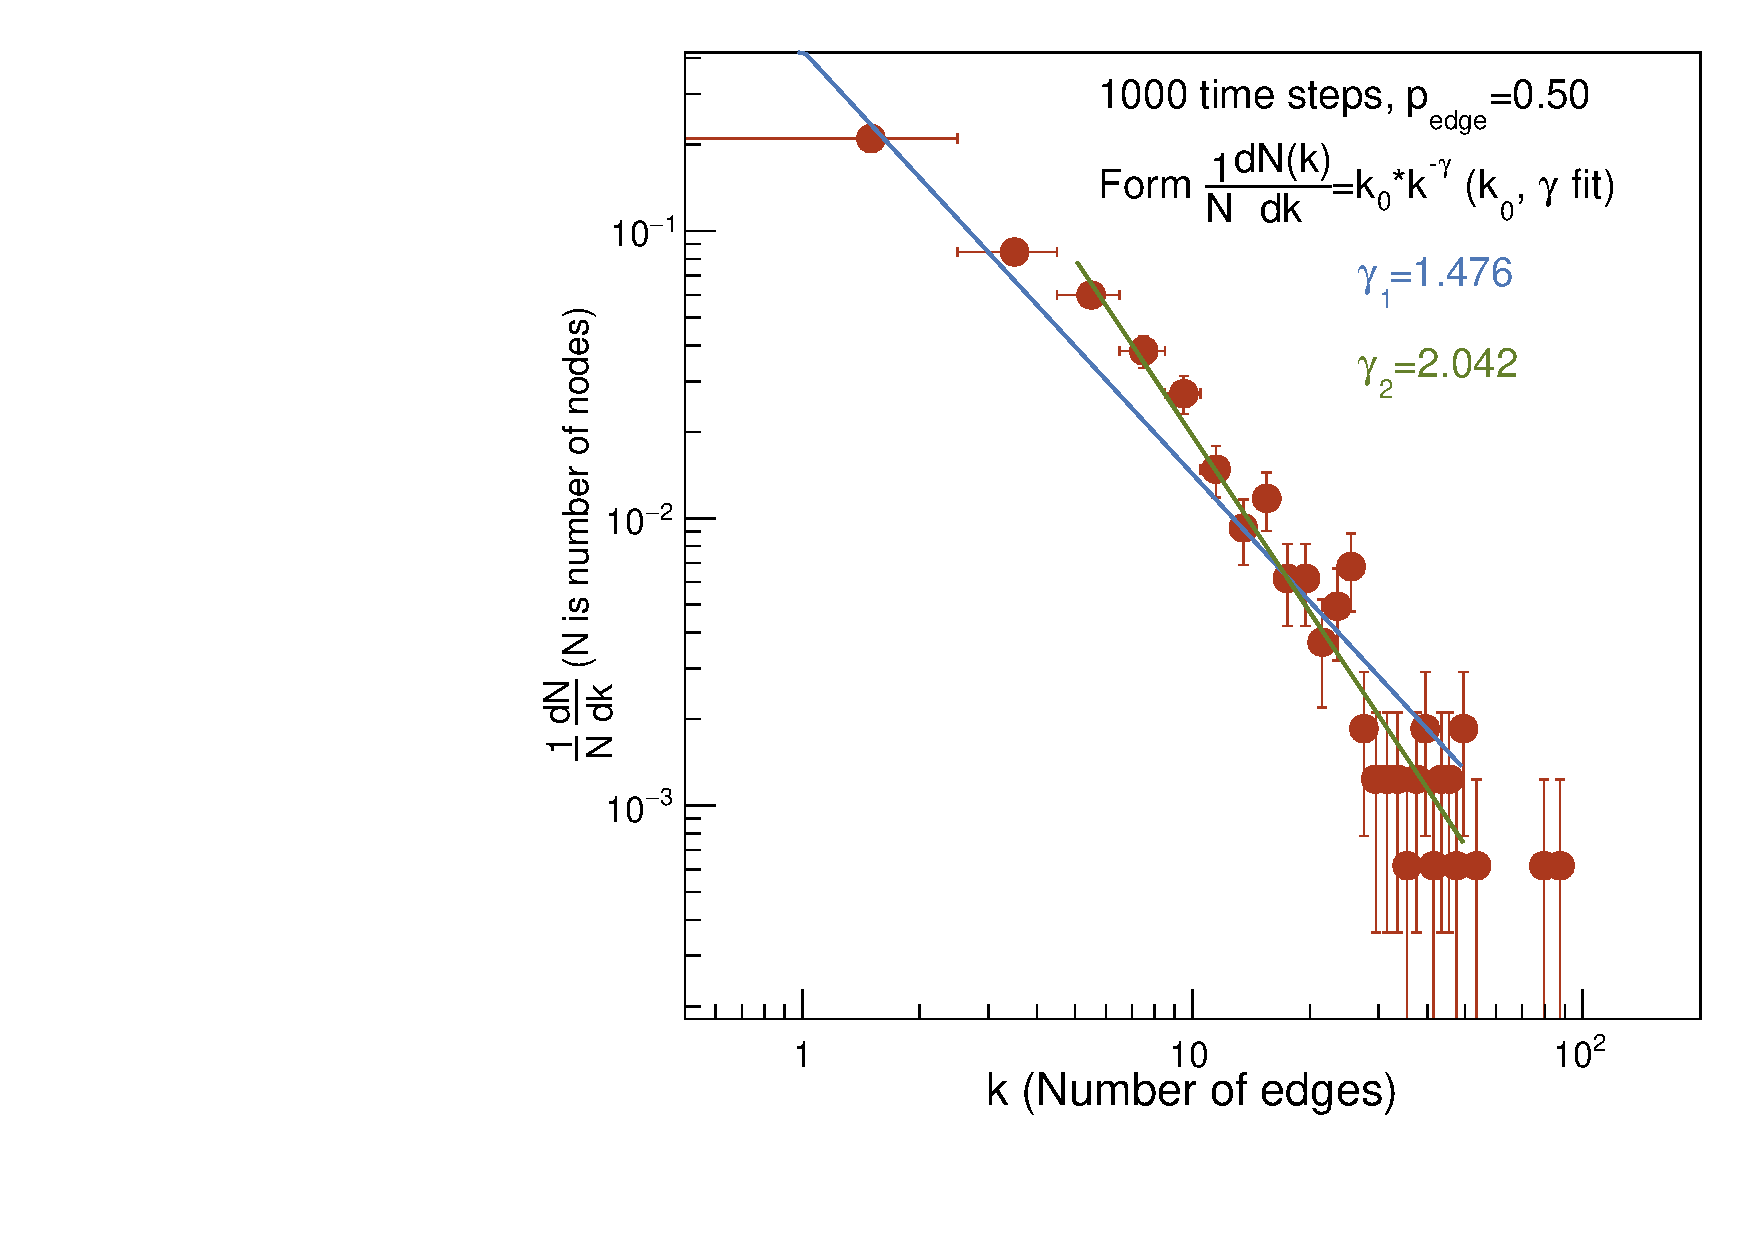
\includegraphics[width=.49\textwidth]{degreeHist_Prob0p500_20171006_112915.pdf} 
    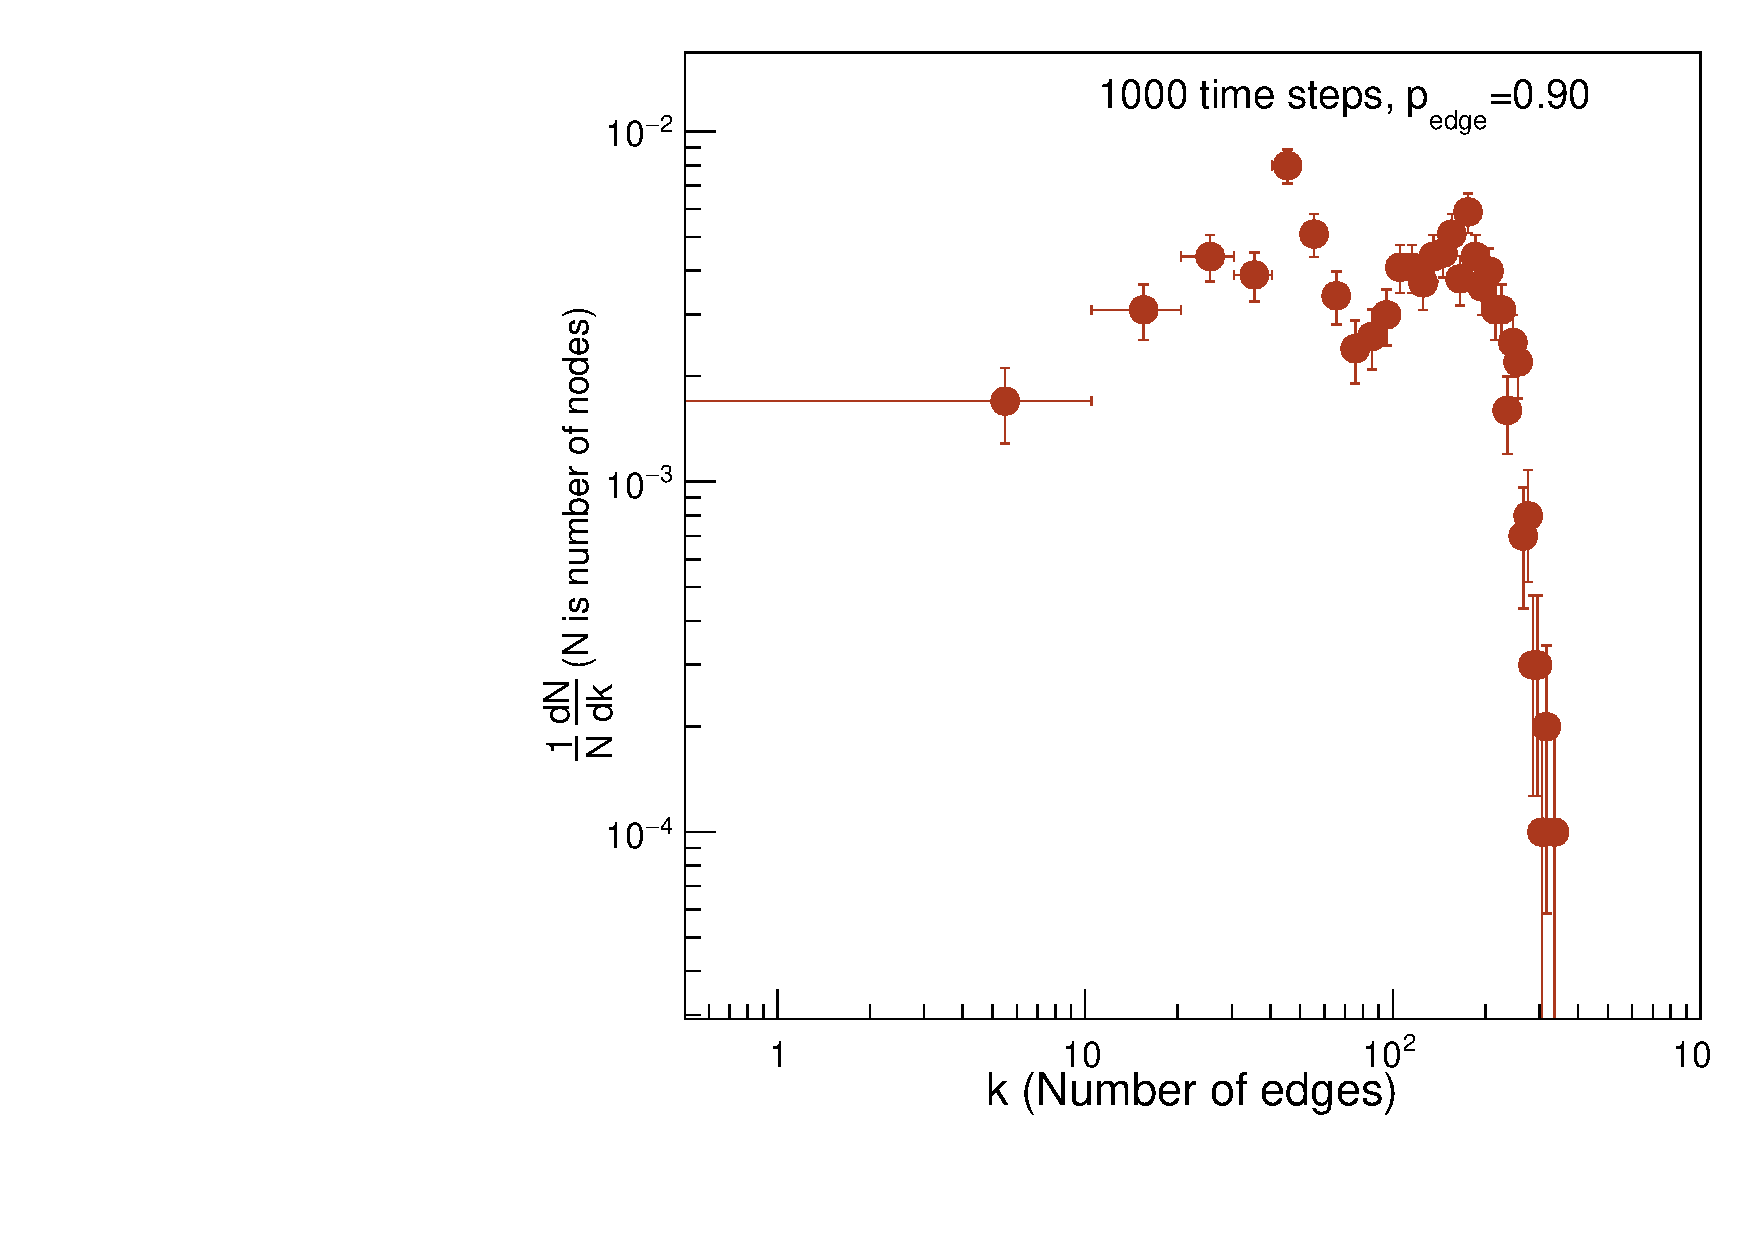
\includegraphics[width=.49\textwidth]{degreeHist_Prob0p900_20171006_112915.pdf} 
    \caption{Distribution for degrees of system when probability of edge forming is 0.5 (left) and 0.9 (right). At probability of 0.5, we find that the system approaches power law behavior. Two fits are attempted of the steeply falling spectrum, one starting at degree k=1 (blue), and another starting at degree k=5 (green). Degree k=5 fit shows better agreement with the simulation. At probability of 0.9, the simulation does not show power law behavior.}
    \label{fig1}
\end{figure}

\begin{figure}[H]
    \centering
    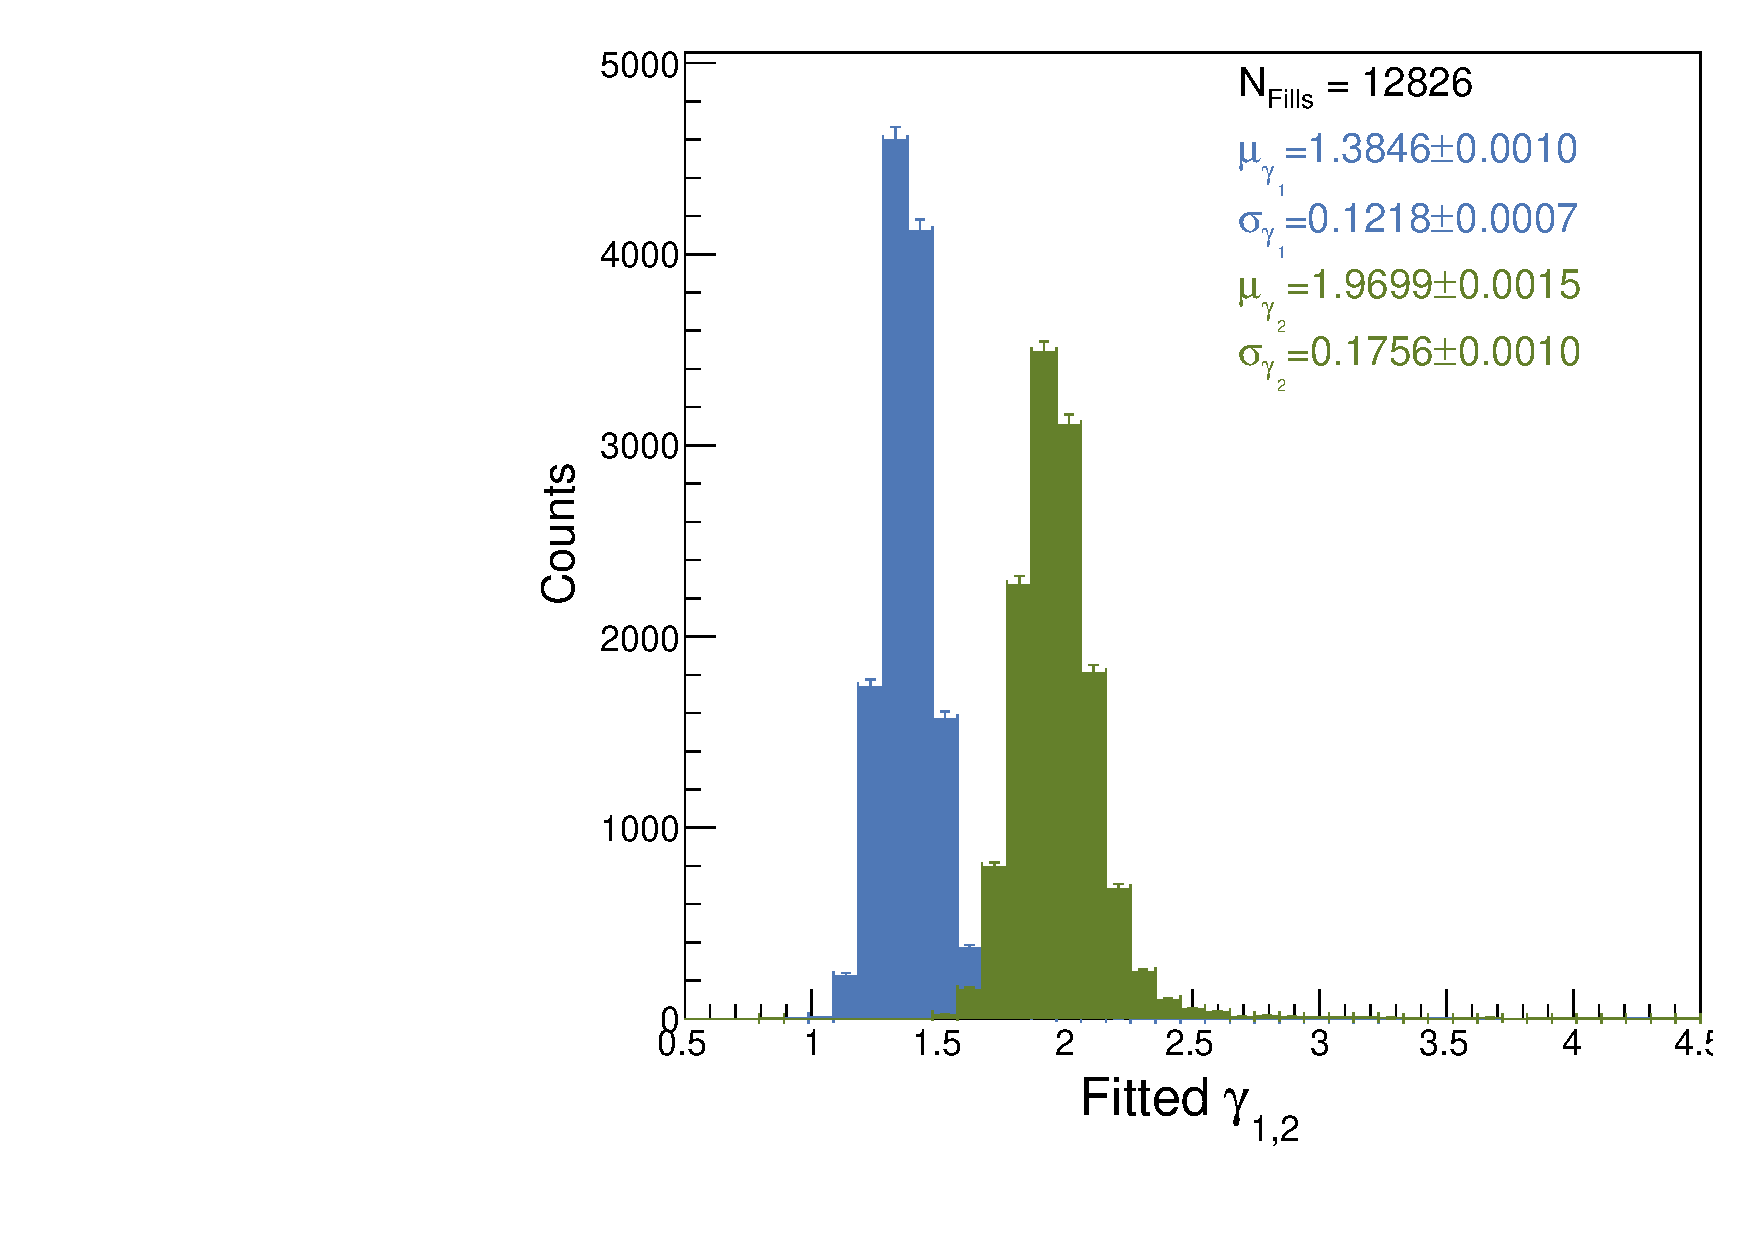
\includegraphics[width=.49\textwidth]{gammaCanv.pdf} 
    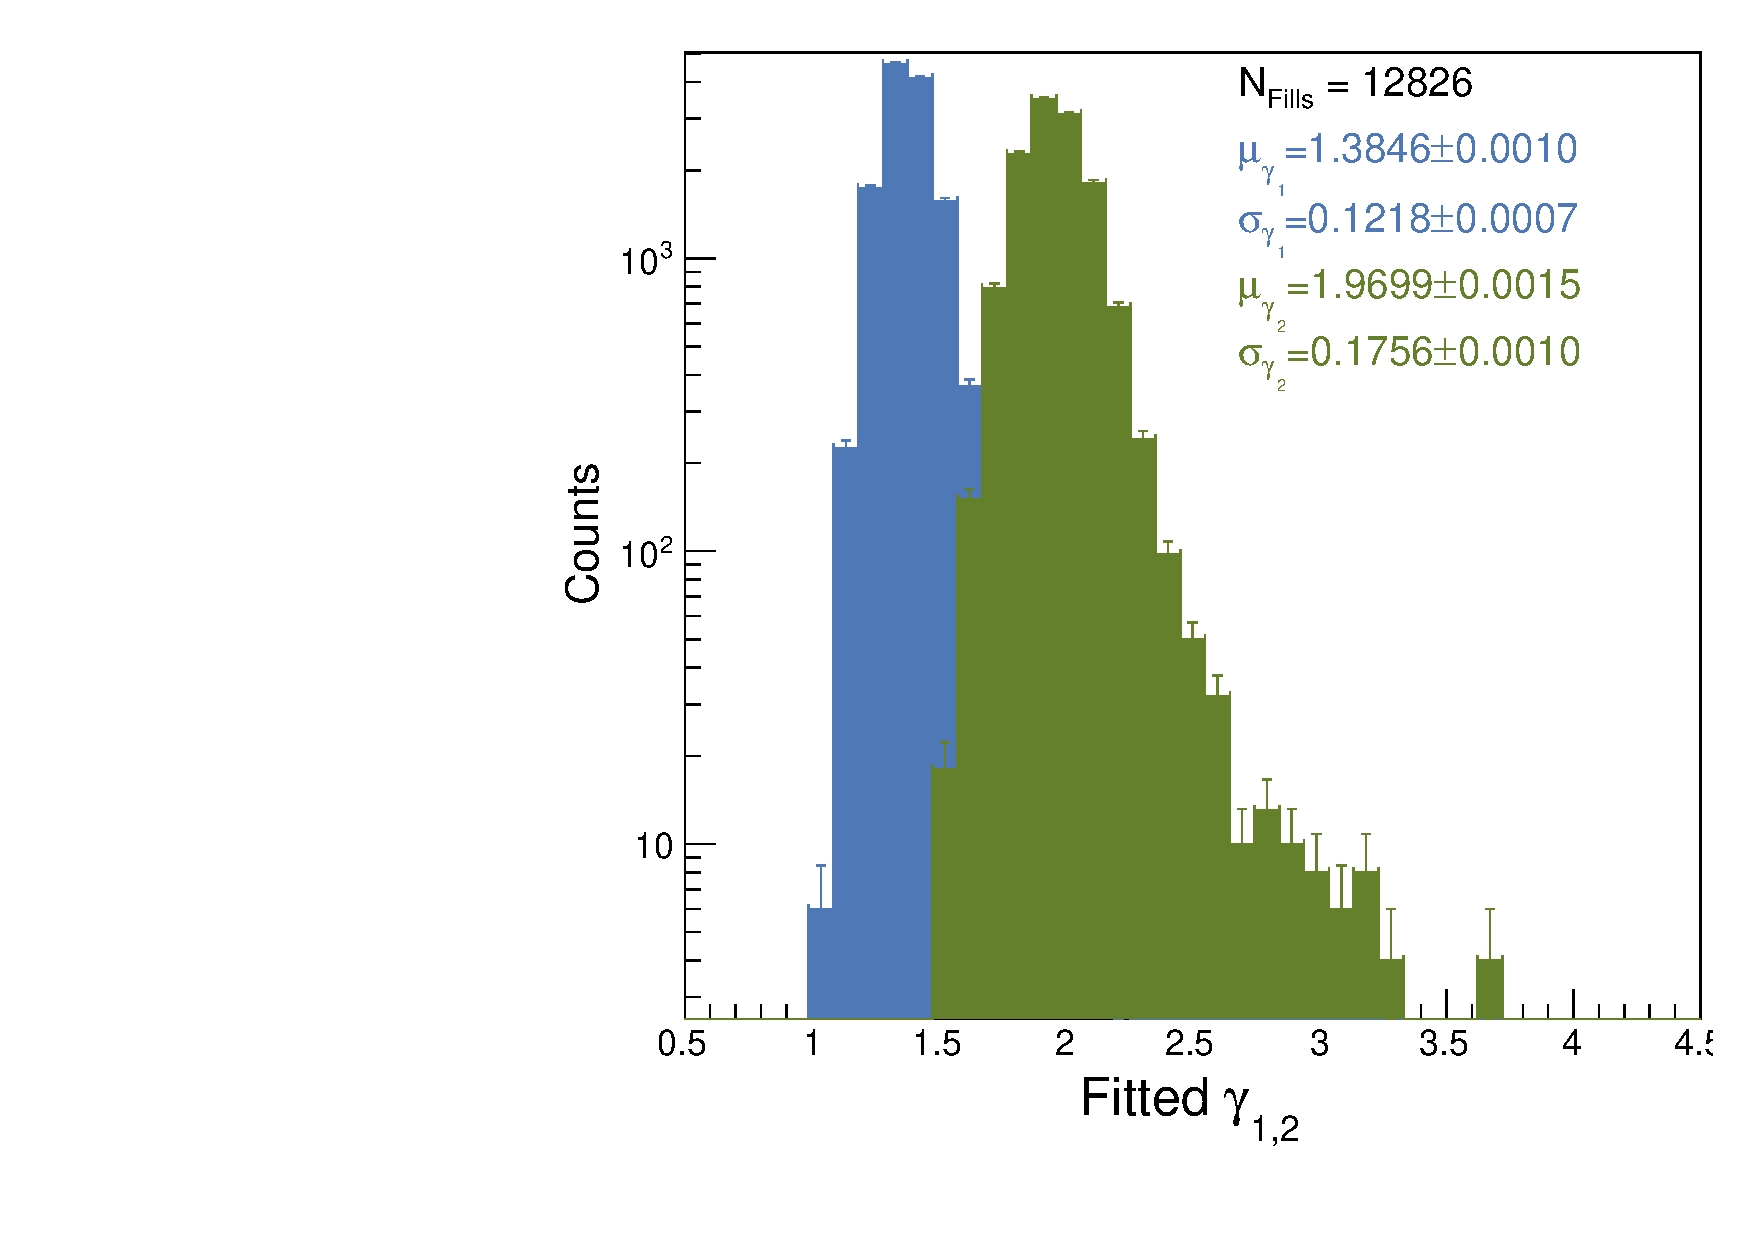
\includegraphics[width=.49\textwidth]{gammaCanv_LOG.pdf} 
    \caption{Fitted $\gamma$ distribution for many simulations taken thru 1000 time steps. Blue corresponds to fits from k=1 to k=50, while green truncates the fit (k=5 to k=50) to try and restrict to the region of least deviation from the power law (cutting out the low k where nodes are first introduced to the network). As can be seen, the central values of these distributions deviate from each other significantly. The green should be taken as the better representation of the power law behavior, with a gamma of about 2. The blue extracted values, while using the full k range where there is data, is a poor model in the low k region. Note the righthand side is a log-scale replot.}
    \label{fig2}
\end{figure}


\section{1.b.4}

If we do not remove 0's then the probability of cloning a zero relative to a non-zero diverges and we are left with an enormous peak at zero (since every zero must clone to be identically another zero). In this case even if you remove the zero peak you will most likely not get to power law behavior in the relatively small number of time steps we use (1000). From the perspective of the system as it might manifest in reality, a cloned node with no edges is no longer a part of the network, and should be excluded in study of the network.

\end{document}

